\documentclass{article}
\usepackage[paperwidth=14in,paperheight=6in,margin=0.22in]{geometry}
\usepackage{xcolor}
\usepackage{tikz}
\renewcommand{\familydefault}{\sfdefault}
\usetikzlibrary{arrows.meta,positioning,calc}

\definecolor{navy}{HTML}{23395B}
\definecolor{bluepanel}{HTML}{EAF1FB}
\definecolor{greenpanel}{HTML}{ECF6F0}
\definecolor{goldpanel}{HTML}{FFF6E5}
\definecolor{rosepanel}{HTML}{FBEDEE}
\pagestyle{empty}

\begin{document}
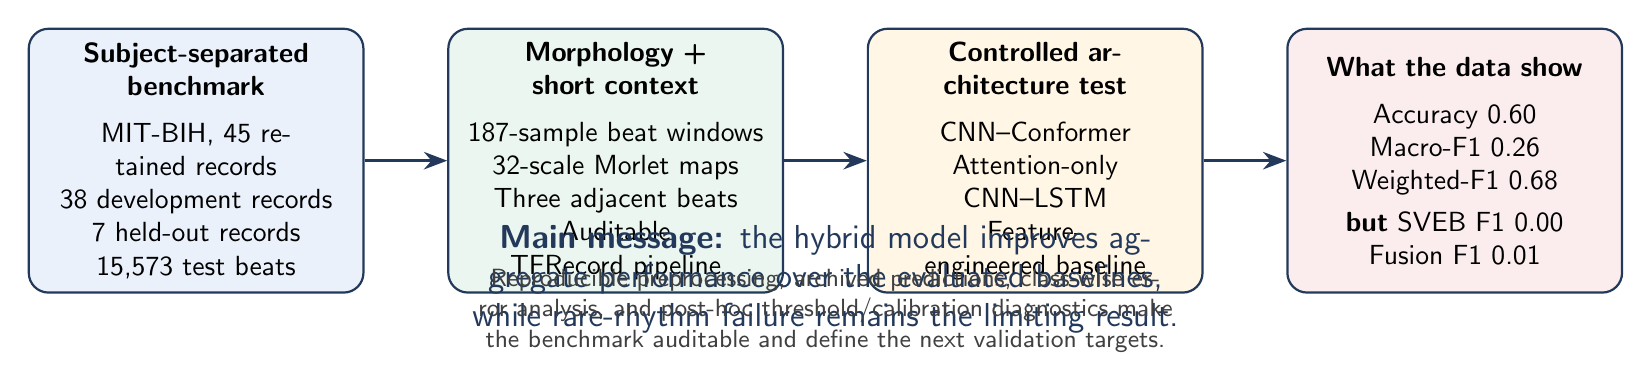
\begin{tikzpicture}[font=\sffamily,>=Stealth,node distance=0.75cm]
  \tikzset{stage/.style={draw=navy,rounded corners=2.5mm,minimum width=4.25cm,minimum height=3.35cm,text width=3.95cm,align=center,line width=0.8pt}}

  \node[stage,fill=bluepanel] (data) {\textbf{Subject-separated benchmark}\\[5pt]
    MIT-BIH, 45 retained records\\
    38 development records\\
    7 held-out records\\
    15{,}573 test beats};

  \node[stage,fill=greenpanel,right=1.05cm of data] (representation) {\textbf{Morphology + short context}\\[5pt]
    187-sample beat windows\\
    32-scale Morlet maps\\
    Three adjacent beats\\
    Auditable TFRecord pipeline};

  \node[stage,fill=goldpanel,right=1.05cm of representation] (model) {\textbf{Controlled architecture test}\\[5pt]
    CNN--Conformer\\
    Attention-only\\
    CNN--LSTM\\
    Feature-engineered baseline};

  \node[stage,fill=rosepanel,right=1.05cm of model] (evidence) {\textbf{What the data show}\\[5pt]
    Accuracy 0.60\\
    Macro-F1 0.26\\
    Weighted-F1 0.68\\[3pt]
    \textbf{but} SVEB F1 0.00\\
    Fusion F1 0.01};

  \draw[->,line width=1.2pt,navy] (data) -- (representation);
  \draw[->,line width=1.2pt,navy] (representation) -- (model);
  \draw[->,line width=1.2pt,navy] (model) -- (evidence);

  \node[below=0.70cm of $(representation)!0.5!(model)$,text width=10.8cm,align=center,text=navy,font=\large]
    {\textbf{Main message:} the hybrid model improves aggregate performance over the evaluated baselines, while rare-rhythm failure remains the limiting result.};

  \node[below=1.25cm of $(representation)!0.5!(model)$,text width=11.3cm,align=center,text=black!75,font=\small]
    {Reproducible preprocessing, archived predictions, class-wise error analysis, and post-hoc threshold/calibration diagnostics make the benchmark auditable and define the next validation targets.};
\end{tikzpicture}
\end{document}
